\chapter{What Is Meditation?}

This chapter follows J. Krishnamurti's San Diego 1970 inquiry into meditation as source material for \emph{How You Got Happiness?}, curated by LazyingArt LLC through Video2Book. There are no validated blackboard frames for this talk, so the visual material here is reconstructed only as compact conceptual notation. The aim is not to turn Krishnamurti into a system-maker, but to make visible the sequence of distinctions by which the talk moves: search, image, recognition, order, control, observation, attention, silence, body, love, sleep, and finally the limit of description.

\section{Before Asking What Meditation Is}

Krishnamurti begins by postponing the question. We are going to ask what meditation is, but before that question can be asked honestly we must ask what we are after. The delay matters. If meditation is made into something to obtain, then it has already joined the ordinary movement of search.

A search is never neutral in this inquiry. To seek truth, God, a perfect life, hope, or companionship is already to carry some contour of what is sought. The mind may not have a sharp definition, but it has an image, a pattern, a recognizable form. Otherwise it would not know that it had found what it was seeking.

We can write the structure in a deliberately simple way:
\begin{equation}
\mathrm{Search}
\longrightarrow
\mathrm{Image}
\longrightarrow
\mathrm{Recognition}
\longrightarrow
\mathrm{AlreadyKnown}.
\end{equation}

This is not a formal psychological theorem. It is a way of preserving the logic of the spoken inquiry. Recognition implies previous knowledge. Therefore a search that depends on recognition remains inside the field of what is already known.

\begin{proposition}
If meditation is approached as a search for a predetermined object, it has already been shaped by desire, image, and recognition.
\end{proposition}

\begin{proof}
To search is to be able, at least vaguely, to recognize the object sought. Recognition presupposes some prior image or memory. Therefore what is sought is not wholly new; it is measured by what the mind already carries. Meditation, in this lecture, cannot begin as another movement toward such an object.
\end{proof}

So the first negative statement is quite severe:
\begin{equation}
\mathrm{Meditation} \Rightarrow \neg \mathrm{Search}.
\end{equation}
Every form of search must come to an end, not because seeking is morally wrong, but because seeking already contains the object it hopes to discover.

\section{Order Without Blueprint}

The next movement is not yet meditation. Krishnamurti says a foundation has to be laid. The foundation is order, or virtue, but he immediately separates it from respectability and from social morality. Order is not conformity to a public standard. It is not produced by authority, personal experience, or a private blueprint.

The lecture's logic is this:
\begin{equation}
\mathrm{Understanding}(\mathrm{Disorder}) \longrightarrow \mathrm{Order}.
\end{equation}

The reverse movement is what must be refused:
\begin{equation}
\mathrm{Order} \neq
f(\mathrm{Blueprint},\mathrm{Authority},\mathrm{Experience},\mathrm{Effort}).
\end{equation}

Disorder exists as long as there is conflict, inwardly and outwardly. Therefore order cannot be imposed by effort, because effort itself belongs to the same field of conflict. We are not adding a better control. We are asking whether disorder can be understood without the distorting movement that tries to conquer it.

\subsection{Question \& Answer}

\paragraph{Question.}
How can order come about without control?

\paragraph{Answer.}
It comes about only through understanding disorder. That means observing conflict as it is, without suppressing it, overcoming it, throttling it, justifying it, or choosing for or against it. The difficulty is that we usually meet disorder with effort, and Krishnamurti's point is that effort distorts the very thing it tries to correct.

The compact relation is:
\begin{align}
\mathrm{Effort} &\longrightarrow \mathrm{Distortion},\\
\mathrm{Observation\ of\ Disorder} &\longrightarrow \mathrm{Understanding},\\
\mathrm{Understanding} &\longrightarrow \mathrm{Order}.
\end{align}

\begin{figure}
\centering
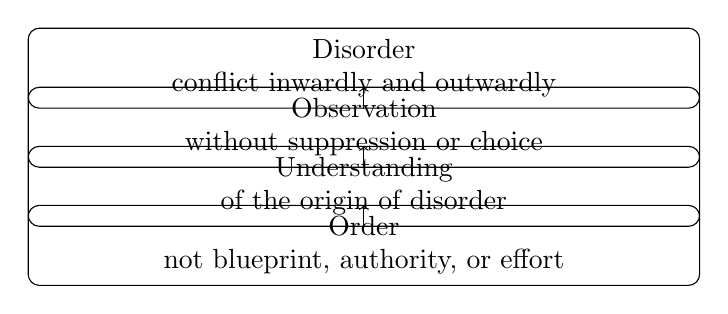
\begin{tikzpicture}[
  node distance=0.75cm,
  every node/.style={draw, rounded corners, align=center, text width=0.68\linewidth, inner sep=4pt},
  every path/.style={->}
]
\node (disorder) {Disorder\\conflict inwardly and outwardly};
\node (observe) [below of=disorder] {Observation\\without suppression or choice};
\node (understand) [below of=observe] {Understanding\\of the origin of disorder};
\node (order) [below of=understand] {Order\\not blueprint, authority, or effort};
\draw (disorder) -- (observe);
\draw (observe) -- (understand);
\draw (understand) -- (order);
\end{tikzpicture}
\caption{A compact reconstruction of the lecture's order-through-understanding movement. No screenshot evidence is available for this diagram.}
\end{figure}

\section{The Controller Is The Controlled}

The ordinary solution to disorder is control. The lecture now turns on that assumption. Control implies suppression, rejection, exclusion, or some division between the one who controls and the thing to be controlled. Once that division appears, conflict appears with it.

The chain is:
\begin{equation}
\mathrm{Control}
\longrightarrow
(\mathrm{Controller}/\mathrm{Controlled})
\longrightarrow
\mathrm{Division}
\longrightarrow
\mathrm{Conflict}
\longrightarrow
\mathrm{Distortion}.
\end{equation}

Krishnamurti's crucial reversal is that the controller is not actually separate from the controlled. The one who says, ``I am angry and I must get rid of anger,'' is not apart from anger. The division is itself part of the disorder.

We can record the identity in the lecture's own conceptual language:
\begin{equation}
\mathrm{Controller}=\mathrm{Controlled},
\qquad
\mathrm{Observer}=\mathrm{Observed}.
\end{equation}

These equalities should not be read as algebra. They are markers for a collapse of false duality. If the observer divides himself from anger, jealousy, despair, or the desire to fulfil, there is contradiction. Where there is contradiction, there is conflict. Where there is conflict, there is distortion.

\begin{remark}
This identity is the hinge of the foundation. Without seeing it, meditation easily becomes another form of self-hypnosis: one fragment of the mind controlling another fragment and calling the struggle spiritual discipline.
\end{remark}

\section{Love, Learning, And Standing Alone}

The foundation now widens. Order alone is not enough if the mind is loveless. Krishnamurti introduces love not as sentiment, not as romance, and not as pleasure. Love is described by negation: it is not touched by pleasure, desire, jealousy, competition, or division between ``my love'' and ``your love.''

The structure can be kept simple:
\begin{equation}
\mathrm{Love}
\neq
g(\mathrm{Pleasure},\mathrm{Desire},\mathrm{Jealousy},\mathrm{Competition},\mathrm{Sentiment}).
\end{equation}

This is also why the talk pauses over discipline. Discipline is not obedience to another. It is learning. And learning, here, means observing oneself: the self-centred activities, the tricks of the mind, the images, the illusions, the romantic ideas, the movement of ``me'' and ``not me.'' Observation is not possible if we look through a formula, a conclusion, or the authority of a psychologist, teacher, group, or organization.

So awareness cannot be handed down. We can be taught words, systems, and practices, but Krishnamurti is asking for a mind that stands alone, unburdened by propaganda and by the experiences of others. The chapter should preserve the severity of this point. It is not an anti-institutional aside; it prepares the rejection of method.

\section{Observation, Exploration, And Experience}

Krishnamurti next separates observation from exploration and experience. Exploration, in this context, involves analysis. Analysis implies an analyser and the thing analysed. Exploration implies an explorer. In each case, a center is accumulating.

Observation is different. It is continuous learning, not continuous accumulation.

\begin{align}
\mathrm{Observation} &\longrightarrow \mathrm{Learning},\\
\mathrm{Exploration} &\longrightarrow \mathrm{Accumulation}
\longrightarrow \mathrm{Action\ from\ Accumulation}.
\end{align}

This distinction is delicate. Rational inquiry is not dismissed. Enquiry may be logical, sane, and critical. But observation, as used here, is not the same as accumulating knowledge from which one later acts.

\subsection{Question \& Answer}

\paragraph{Question.}
Why do we want deeper and wider experiences?

\paragraph{Answer.}
Because ordinary life often feels small, petty, fearful, and burdened. The craving for marvellous experience can become an escape from what is. But experience requires recognition. If we know an experience as pleasant, noble, mystical, spiritual, or beautiful, then recognition has already entered. Recognition belongs to the past.

The derivation is:
\begin{enumerate}
\item Experience must be recognized as experience.
\item Recognition depends on what is already known.
\item What is already known is the past.
\item Therefore experience, as recognized experience, is not wholly new.
\item The craving for greater experience is often an escape from what is.
\end{enumerate}

In symbols:
\begin{equation}
\mathrm{Experience}
\longrightarrow
\mathrm{Recognition}
\longrightarrow
\mathrm{Past}.
\end{equation}

And:
\begin{equation}
\mathrm{Craving\ for\ Experience}
\longrightarrow
\mathrm{Escape\ from\ What\ Is}.
\end{equation}

This is why the talk can return to meditation only after method, purpose, search, and experience have been put aside. Otherwise meditation becomes another refined appetite.

\section{Meditation Without Method}

Now the original question returns: what is meditation? Krishnamurti refuses the familiar answer. Meditation is not sitting for ten minutes, fixing the mind on an image, repeating a formula, or battling to control thought. Any system soon becomes repetitive and mechanical. If we practise a method, we become what the method offers; and what a method offers is not truth, because truth is living while method is mechanical.

The compact chain is:
\begin{equation}
\mathrm{Method}
\longrightarrow
\mathrm{Practice}
\longrightarrow
(\mathrm{Practitioner}/\mathrm{Practised})
\longrightarrow
\mathrm{Division}
\longrightarrow
\mathrm{Conflict}
\longrightarrow
\mathrm{Disorder}.
\end{equation}

The important point is the reappearance of division. The same structure that made control disorderly also makes practice disorderly when practice is taken as a path toward truth.

What, then, is the positive movement? The mind that observes must be quiet. Not quiet because it has been forced into quietness, but quiet because clear seeing requires quietness. If we are to listen completely, we cannot simultaneously translate, compare, condemn, judge, or drift elsewhere.

\begin{equation}
\mathrm{Necessity\ to\ See\ Clearly}
\longrightarrow
\mathrm{Quiet\ Mind}.
\end{equation}

This is the opposite of cultivating silence in time. To cultivate a still mind would introduce the cultivator, the goal, and time. That is the old duality in a subtler form.

\subsection{Question \& Answer}

\paragraph{Question.}
If attention is not practised, what happens when the mind wanders?

\paragraph{Answer.}
We do not battle with wandering. We know inattention as inattention. The very awareness of inattention is attention. But if action comes out of that inattention, that action too must be seen.

A compact rule, not a technique, is:
\begin{align}
\mathrm{Practice}(\mathrm{Attention}) &\longrightarrow \mathrm{Inattention},\\
\mathrm{Awareness}(\mathrm{Inattention}) &\longrightarrow \mathrm{Attention}.
\end{align}

This is the closest the lecture comes to an update rule, but it must not be turned into one. The point is not to perform a procedure. The point is to see without choice.

\section{The Still Body, Joy, And Attention In Sleep}

Silence of mind is not isolated from the body. Krishnamurti extends the inquiry to the organism: fidgeting, restless movement, bodily insensitivity, compulsion, overindulgence, and the dulling action of pleasure. The body, he says, has its own intelligence, which thought spoils when it pursues pleasure or forces the organism.

We should handle this carefully and not expand it into physiology. The lecture's claim is practical and inward: a sensitive body, a quiet mind, and love without pleasure-distortion belong together.

\begin{equation}
\mathrm{Still\ Body}
+
\mathrm{Quiet\ Mind}
+
\mathrm{Love\ without\ Pleasure\text{-}Distortion}
\longrightarrow
\mathrm{Harmony}.
\end{equation}

Pleasure and joy are then separated:
\begin{align}
\mathrm{Pleasure} &\longrightarrow \mathrm{Motive},\\
\mathrm{Joy} &\longrightarrow \neg \mathrm{Motive}.
\end{align}

Joy cannot be held by saying, ``I am joyous.'' The moment one seeks its cause in order to repeat it, it is no longer joy in the sense intended here.

\subsection{Question \& Answer}

\paragraph{Question.}
What is the point of such a life?

\paragraph{Answer.}
Krishnamurti answers by questioning the one who asks. If the question comes as a demand for utility, then this kind of life has no point in that market of usefulness. But if this harmony is actually alive, then it is not a means to something else. It is everything: teacher, disciple, neighbour, cloud, beauty, and love are no longer divided in the old way.

The final movement concerns sleep. The waking mind, with all its daily activity, usually continues in sleep. Dreams are treated here as the continuation of the same movement: action, anxiety, self-centredness, fear, guilt, interpretation. But if thought is watched during the day, then sleep is not merely the continuation of unattended disorder.

\begin{equation}
\mathrm{Attention}_{\mathrm{day}}
\longrightarrow
\mathrm{Attention}_{\mathrm{sleep}}
\longrightarrow
\mathrm{Whole\ Mind\ Awake}.
\end{equation}

This should not be presented as sleep science. It is the lecture's final extension of attention. Attention is not only a waking discipline; when the mind is attentive during the day, Krishnamurti says there is attention in sleep.

Beyond that point the lecture refuses description. Every form of description is not the described:
\begin{equation}
\mathrm{Description} \neq \mathrm{Described}.
\end{equation}

One can point to the door. One cannot describe what is beyond it and still be faithful to the inquiry.

\section{Summary}

The lecture does not define meditation by offering a method. It approaches meditation by clearing away what meditation is not: search, predetermined image, hope as escape, imposed order, control, authority, practice, accumulated experience, and cultivated silence. The structure is negative, but not empty. Through negation it uncovers a precise movement: observe disorder without distortion; see the controller as the controlled and the observer as the observed; distinguish observation from exploration and experience; listen without translation; know inattention without battle; allow quietness to arise from the necessity of seeing clearly.

Meditation, in this chapter's notation, begins where search ends:
\begin{equation}
\mathrm{Meditation}
\Rightarrow
\neg \mathrm{Search},
\qquad
\mathrm{Attention}
\not\equiv
\mathrm{Practice}.
\end{equation}

The final claim is deliberately restrained. When body, mind, brain, and heart are in harmony, attention extends even into sleep; but beyond the whole mind being awake, description fails. The chapter should therefore close as the lecture closes: not with a doctrine, but with the understanding that pointing is possible and possession is not.